\documentclass[]{exam}
\usepackage{amssymb}
\usepackage{amsfonts}
\usepackage{amsmath}
\usepackage{amsthm}
\usepackage[top=1in, bottom=1.5in, left=1in, right=1in]{geometry}
\usepackage{tikz}
\usepackage{pgfplots}
\usepackage{empheq}
\usepackage{mathrsfs}
\checkboxchar{$\Box$}
\usepackage{graphicx}
\usepackage{caption}
\usepackage{float}
\usepackage{enumerate}
\usepackage{comment}
\usepackage{multicol}
\usepackage{color}
\usepackage{advdate}
\usepackage{gensymb}
\usetikzlibrary{arrows}
\usepackage{multirow}
\usepackage{arydshln}
\usepackage{verbatim}

\usepackage{pgfkeys,pgfcalendar}

\newcount\pgfdatecount
\newcommand{\tomorrow}{%
\pgfcalendardatetojulian{\year-\month-\day+1}{\pgfdatecount}
\pgfcalendarjuliantodate{\the\pgfdatecount}{\myyear}{\mymonth}{\myday}
\pgfcalendarmonthname{\mymonth}\space\myday,\space\myyear%
}

\newcommand{\advanceday}[1][1]{
\begingroup
\AdvanceDate[#1]
\today
\endgroup}

\newcommand{\vertex}{\node[vertex]}
\tikzstyle{vertex}=[circle, draw, inner sep=0pt, minimum size=6pt]
\usepackage{lastpage} 
\usepackage{extramarks}
\usepackage{graphicx} 
\usepackage{tikz}
\usepackage{sectsty} 
\usepackage{amsmath,amsfonts,amsthm} 
\usepackage{wrapfig, blindtext}

% Margins
\topmargin=-0.45in
\evensidemargin=0in
\oddsidemargin=0in
\textwidth=6.5in
\textheight=9.0in
\headsep=0.25in 
\numberwithin{equation}{section}
\linespread{1.1} 
\setlength\parindent{0pt} 
\setlength\answerskip{-.075in}
\setlength\answerlinelength{.5in}
\newcommand{\myitem}{\item[-]}

% HEADER AND FOOTER
\pagestyle{headandfoot}
\runningheadrule
\runningfootrule
\firstpageheader{Kutztown University}{  }{MATH 210}
\firstpageheadrule
\runningheader{P3.HW}{ }{MATH 210}
\firstpagefooter{}{}{} 
\runningfooter{}{}{Page \thepage\ of \numpages}

\captionsetup{width=.75\textwidth}


% TITLE PAGE
\newcommand{\assignmentname}{Phase 3 -- Homework} % Assignment title
\newcommand{\coursetitle}{MATH 210 -- Mathematical Computing and Typesetting}
\newcommand{\duedate}{Due: Friday, April 10 by 11:59 PM on D2L} % Update as needed
\newcommand{\readsections}{\, } % Teacher/lecturer
\newcommand{\semester}{\, }
\title{
\vspace{2in}
\textmd{\textbf{\course:\ \assignmentname}}\\
\normalsize\vspace{0.1in}{\duedate}\\
\vspace{0.1in}\large{\textit{\instructor}}
\vspace{3in}
}
\author{\textbf{Author: \authorname}}
\date{Last Updated: \today}

\pointsinrightmargin
\bracketedpoints



\begin{document}
%%%%%%%%%%%%%%%%%%%%%%%%%%%%%%%%%%%%%%%%%%%%%%%%%%%%%
% COMPILE TITLES AND SUCH
%%%%%%%%%%%%%%%%%%%%%%%%%%%%%%%%%%%%%%%%%%%%%%%%%%%%%
\hspace{1in}\\ \vspace{.15in}


\begin{center}
\normalsize
 \fbox{\fbox{\parbox{5.5in}{
        {\bf Instructions:}  Upload the \texttt{tex} file for this document to your Overleaf project.  All solutions shall be completed on this packet by typing your solution in \LaTeX\, in the space provided.  All solutions should be detailed and should clearly demonstrate the process by which you arrived at the answer.  Submit the compiled \texttt{pdf} file to D2L by 11:59 PM on the due date below.  Submit only a single pdf file of your entire packet.  The question will also ask you to make calculations in Python.  Upload any Python files to the appropriate folder in your GitHub repository.  In this folder, a \texttt{py} file is to be submitted for each problem such that when the \texttt{py} file is executed, the output (as presented in Python) is the solution to the problem. Academic dishonesty will not be tolerated.  }}}
\end{center}

\vspace{.5cm}

\begin{center}
	\Huge\textsc{
	\assignmentname}\\[4pt]
        \Large{\textsc{\coursetitle}\\[10pt]}
        \Large{\textsc{\duedate}\\[8pt]}
        \Large{\textsc{\readsections}\\[8pt]}
\end{center}

\vspace{1cm}

%%%%%%%%%%%%%%%%%%%%%%%%%%%%%%%%%%%%%%
% Uncomment the syntax below when you type up the solutions and type 
% your name.
\begin{center}
	\large{\textsc{\textcolor{red}{Solutions by Brooks Emerick}}}
\end{center}
\vfill

%%%%%%%%%%%%%%%%%%%%%%%%%%%%%%%%%%%%%%
% Reminders:
%%%%%%%%%%%%%%%%%%%%%%%%%%%%%%%%%%%%%%
Remember to begin each \texttt{py} file with \texttt{import numpy as np} and \verb|import matplotlib.pyplot as plt|.  
For this assignment you will also need \texttt{import networkx as nx}.  
If you compute eigenvalues/eigenvectors in Python, you may use \texttt{np.linalg.eig}.  

% Blank Page
\clearpage

\begin{questions}
%%%%%%%%%%%%%%%%%%%%%%%%%%%%%%%%%%%%%%
% NUMBER 1 
%%%%%%%%%%%%%%%%%%%%%%%%%%%%%%%%%%%%%%
\question Consider the matrix
\[
A=\begin{bmatrix}
5 & 2\\
1 & 2
\end{bmatrix}.
\]

\begin{parts}
\part Compute the characteristic polynomial $\det(A-\lambda I)$ and find the eigenvalues of $A$.  Type your work explicitly below. \\

The matrix $A - \lambda I$ is given by 
\[ \begin{bmatrix} 5-\lambda & 2 \\ 1 & 2-\lambda \end{bmatrix} \]
and the characteristic polynomial is 
\[ \det(A - \lambda I) = (5-\lambda)(2 - \lambda) - (2)(1) = 8 -7\lambda + \lambda^2. \]
The eigenvalues are found by computing the roots of the characteristic polynomial: 
\begin{align*}
\lambda^2 - 7 \lambda + 8 = 0 \quad & \Rightarrow \quad \lambda_{1,2} = \frac{7 \pm \sqrt{7^2 - 4(1)(8)}}{2} \\ 
& \Rightarrow \quad \lambda_{1,2} = \frac{7 \pm  \sqrt{17}}{2} \end{align*}

Therefore, the two eigenvalues are 
\[ \lambda_{1} = \frac{7 - \sqrt{17}}{2} \qquad \lambda_2 = \frac{7 + \sqrt{17}}{2}. \]

\part For each eigenvalue, find a corresponding eigenvector.  Type your work explicitly below and clearly label which eigenvector corresponds to which eigenvalue. \\

We let the eigenvector $\boldsymbol{v}_i$ correspond to eigenvalue $\lambda_i$ for $i = 1, 2$.  To determine both eigenvectors simultaneously, we solve the equation 
\[ A \boldsymbol{v} = \lambda \boldsymbol{v}, \qquad \Rightarrow \qquad \begin{bmatrix} 5 & 2 \\ 1 & 2 \end{bmatrix} \begin{bmatrix} x \\ y \end{bmatrix} = \begin{bmatrix} \lambda x \\ \lambda y \end{bmatrix} \]
for some non-trivial vector $\boldsymbol{v}$.  Writing this using two equations gives the following: 
\begin{align*}
	\begin{cases}
		5x + 2y = \frac{7 \pm  \sqrt{17}}{2}x \\ 
		x + 2y = \frac{7 \pm  \sqrt{17}}{2}y \end{cases} & = 
	\begin{cases} 
		\left( 5 - \frac{7 \pm  \sqrt{17}}{2}\right)x + 2y = 0 \\ 
		x + \left( 2 -  \frac{7 \pm  \sqrt{17}}{2}\right)y = 0 \end{cases} \\ 
		& =
	\begin{cases} 
		\frac{3 \mp \sqrt{17}}{2} x + 2y = 0 \\ 
		x + \frac{-3 \mp \sqrt{17}}{2}y = 0 \end{cases} \\
		& =
	\begin{cases} 
		x = \frac{-2}{\frac{3 \mp \sqrt{17}}{2} }y \\ 
		x =\frac{3 \pm \sqrt{17}}{2}y  \end{cases} \\ 
		& = 
	\begin{cases} 
		x = \frac{-4}{3 \mp \sqrt{17} }y \\ 
		x =\frac{3 \pm \sqrt{17}}{2}y  \end{cases} \\ 
		& = 
		\begin{cases} 
		x = \frac{-4(3 \pm \sqrt{17})}{-8 }y \\ 
		x =\frac{3 \pm \sqrt{17}}{2}y  \end{cases} \\ 
		&=
	\begin{cases} 
		x = \frac{3 \pm \sqrt{17}}{2}y \\ 
		x =\frac{3 \pm \sqrt{17}}{2}y  \end{cases}\end{align*}

From this, we can construct each eigenvector:
\[ \boldsymbol{v}_1 = \begin{bmatrix} \frac{3- \sqrt{17}}{2} \\ 1 \end{bmatrix}, \qquad \boldsymbol{v}_2 = \begin{bmatrix} \frac{3 + \sqrt{17}}{2} \\ 1 \end{bmatrix}. \]
\part Verify your answers by checking that $A\mathbf{v}=\lambda \mathbf{v}$ for each eigenpair $(\lambda,\mathbf{v})$. \\ 

To check our answers, we can check the equation $A\boldsymbol{v}_i = \lambda_i \boldsymbol{v}_i$ for $i = 1, 2$.  For the left side of this equation, we have 
\begin{align*} 
A \boldsymbol{v}_1 & = \begin{bmatrix} 5 & 2 \\ 1 & 2 \end{bmatrix} \begin{bmatrix} \frac{3- \sqrt{17}}{2} \\ 1 \end{bmatrix} \\ 
	& = \begin{bmatrix} 5\left(  \frac{3- \sqrt{17}}{2} \right) + 2 (1) \\ \left( \frac{3- \sqrt{17}}{2} \right) + 2 (1) \end{bmatrix} \\ 
	& = \begin{bmatrix}  \frac{15- 5\sqrt{17}}{2} +2 \\  \frac{3- \sqrt{17}}{2}  + 2 \end{bmatrix} \\
	& = \begin{bmatrix}  \frac{19- 5\sqrt{17}}{2}  \\  \frac{7- \sqrt{17}}{2}  \end{bmatrix}.\end{align*}
The right hand side of the equation gives 
\begin{align*} 
\lambda_1 \boldsymbol{v}_1 & = \left(\frac{7 - \sqrt{17}}{2}\right) \begin{bmatrix} \frac{3- \sqrt{17}}{2} \\ 1 \end{bmatrix} \\ 
	& = \begin{bmatrix} \left(\frac{7 - \sqrt{17}}{2}\right)\left(\frac{3- \sqrt{17}}{2}\right) \\ \frac{7 - \sqrt{17}}{2} \end{bmatrix} \\ 
	& = \begin{bmatrix} \frac{21 - 7\sqrt{17} - 3\sqrt{17} + 17 }{4} \\  \frac{7 - \sqrt{17}}{2} \end{bmatrix} \\ 
	& = \begin{bmatrix} \frac{38 - 10\sqrt{17} }{4} \\  \frac{7 - \sqrt{17}}{2} \end{bmatrix}\\
	& = \begin{bmatrix} \frac{19 - 5\sqrt{17} }{2} \\  \frac{7 - \sqrt{17}}{2} \end{bmatrix}\end{align*}
We can see directly that the equation $A\boldsymbol{v}_1 = \lambda_1 \boldsymbol{v}_1$.  Checking the other eigenpair, we have 
\begin{align*} 
A \boldsymbol{v}_2 & = \begin{bmatrix} 5 & 2 \\ 1 & 2 \end{bmatrix} \begin{bmatrix} \frac{3+ \sqrt{17}}{2} \\ 1 \end{bmatrix} \\ 
	& = \begin{bmatrix} 5\left(  \frac{3+\sqrt{17}}{2} \right) + 2 (1) \\ \left( \frac{3+\sqrt{17}}{2} \right) + 2 (1) \end{bmatrix} \\ 
	& = \begin{bmatrix}  \frac{15+ 5\sqrt{17}}{2} +2 \\  \frac{3+ \sqrt{17}}{2}  + 2 \end{bmatrix} \\
	& = \begin{bmatrix}  \frac{19+5\sqrt{17}}{2}  \\  \frac{7+ \sqrt{17}}{2}  \end{bmatrix},\end{align*}
and 
\begin{align*} 
\lambda_2 \boldsymbol{v}_2 & = \left(\frac{7 + \sqrt{17}}{2}\right) \begin{bmatrix} \frac{3+ \sqrt{17}}{2} \\ 1 \end{bmatrix} \\ 
	& = \begin{bmatrix} \left(\frac{7 + \sqrt{17}}{2}\right)\left(\frac{3+\sqrt{17}}{2}\right) \\ \frac{7 + \sqrt{17}}{2} \end{bmatrix} \\ 
	& = \begin{bmatrix} \frac{21 + 7\sqrt{17} + 3\sqrt{17} + 17 }{4} \\  \frac{7 + \sqrt{17}}{2} \end{bmatrix} \\ 
	& = \begin{bmatrix} \frac{38 + 10\sqrt{17} }{4} \\  \frac{7 +  \sqrt{17}}{2} \end{bmatrix}\\
	& = \begin{bmatrix} \frac{19 + 5\sqrt{17} }{2} \\  \frac{7 + \sqrt{17}}{2} \end{bmatrix}.\end{align*}
We have shown that the eigenpairs satisfy the definition.  


\part In a Python file, define $A$ as a NumPy array.  Use \texttt{np.linalg.eig} to compute eigenvalues and eigenvectors.  Print the eigenvalues/eigenvectors.\\

The eigenvalues are approximated as 
\[ \lambda_{1} = \frac{7 - \sqrt{17}}{2} \approx 1.4384  \qquad \lambda_2 = \frac{7 + \sqrt{17}}{2} \approx 5.5616. \]
We can normalize the eigenvectors and present them as unit vectors with an approximation to the components.  This way, we can compare our exact result to the output of the Python computation.  The length of $\boldsymbol{v}_1$ is given by the following 
\[ |\boldsymbol{v}_{1}| = \sqrt{\left( \frac{3-\sqrt{17}}{2}\right)^2 + 1^2} = \sqrt{\frac{9 - 6\sqrt{17} + 17}{4} + 1} =  \sqrt{\frac{26 - 6\sqrt{17} + 4}{4} }  = \sqrt{\frac{15 - 3\sqrt{17}}{2}}.\]
The length of $\boldsymbol{v}_2$ is given by 
\[ |\boldsymbol{v}_{2}| = \sqrt{\left( \frac{3+\sqrt{17}}{2}\right)^2 + 1^2} = \sqrt{\frac{9 + 6\sqrt{17} + 17}{4} + 1} = \sqrt{\frac{26 + 6\sqrt{17} + 4}{4} } = \sqrt{\frac{15 + 3\sqrt{17}}{2}}.\]
Finding the two unit eigenvectors gives: 
\begin{align*}
	\boldsymbol{u}_1 = \frac{\boldsymbol{v}_1}{|\boldsymbol{v}_1|} & = \begin{bmatrix} \frac{\frac{3- \sqrt{17}}{2}}{\sqrt{\frac{15 - 3\sqrt{17}}{2}}} \\ \frac{1}{\sqrt{\frac{15 - 3\sqrt{17}}{2}}} \end{bmatrix}  = \begin{bmatrix} \frac{3 - \sqrt{17}}{\sqrt{30-6\sqrt{17}}} \\ \frac{\sqrt{2}}{\sqrt{15 - 3\sqrt{17}}} \end{bmatrix} \approx \begin{bmatrix} -0.4896 \\ 0.8719 \end{bmatrix} \\ 
	\boldsymbol{u}_2 = \frac{\boldsymbol{v}_2}{|\boldsymbol{v}_2|} & = \begin{bmatrix} \frac{\frac{3+\sqrt{17}}{2}}{\sqrt{\frac{15 + 3\sqrt{17}}{2}}} \\ \frac{1}{\sqrt{\frac{15 + 3\sqrt{17}}{2}}} \end{bmatrix}  = \begin{bmatrix} \frac{3 + \sqrt{17}}{\sqrt{30+6\sqrt{17}}} \\ \frac{\sqrt{2}}{\sqrt{15 + 3\sqrt{17}}} \end{bmatrix} \approx \begin{bmatrix} 0.9628 \\ 0.2703\end{bmatrix} \end{align*}

Using the \texttt{np.linalg.eig} package in Python, we obtain the following numerical results for the eigenvalues: 
\[ \lambda_{1} \approx 5.5616 \qquad \lambda_2  \approx 1.4384,\]
which is consistent with our solution.  Furthermore, Python outputs the following matrix, whose columns are the eigenvectors: 
\[ \begin{bmatrix}0.9628 & -0.4896\\ 0.2703 & 0.8719  \end{bmatrix}, \]
which is also consistent with our solution.


\end{parts}

\pagebreak

%%%%%%%%%%%%%%%%%%%%%%%%%%%%%%%%%%%%%%
% NUMBER 2
%%%%%%%%%%%%%%%%%%%%%%%%%%%%%%%%%%%%%%
\question Consider the following three matrices.  

Let the nodes be
\[
\{A,B,C,D,E\}.
\]
You are given three symmetric weighted adjacency matrices:
\[
A_{\text{strong}}=
\begin{bmatrix}
0 & 4 & 2 & 0 & 0\\
4 & 0 & 1 & 2 & 0\\
2 & 1 & 0 & 3 & 0\\
0 & 2 & 3 & 0 & 2\\
0 & 0 & 0 & 2 & 0
\end{bmatrix},
\qquad
A_{\text{medium}}=
\begin{bmatrix}
0 & 0 & 0 & 2 & 0\\
0 & 0 & 1 & 1 & 3\\
0 & 1 & 0 & 0 & 1\\
2 & 1 & 0 & 0 & 0\\
0 & 3 & 1 & 0 & 0
\end{bmatrix},
\qquad
A_{\text{weak}}=
\begin{bmatrix}
0 & 0 & 1 & 0 & 1\\
0 & 0 & 0 & 0 & 0\\
1 & 0 & 0 & 0 & 2\\
0 & 0 & 0 & 0 & 1\\
1 & 0 & 2 & 1 & 0
\end{bmatrix}.
\]

Define the combined interaction matrix
\[
A(\alpha)=A_{\text{strong}}+\alpha A_{\text{medium}}+\alpha^2 A_{\text{weak}}.
\]

\begin{parts}

\part Compute the strength of \emph{every} node, $s_A(\alpha),s_B(\alpha),s_C(\alpha),s_D(\alpha),s_E(\alpha)$, and simplify each expression.  Type them below. \\

The node strength is the column sum of the resulting matrix $A(\alpha)$.  This gives the following: 
\begin{align*}
s_A(\alpha) & = 6 + 2\alpha + 2\alpha^2\\
s_B(\alpha) & = 7 + 5\alpha\\
s_C(\alpha) & = 6 + 2\alpha + 3\alpha^2\\
s_D(\alpha) & = 7 + 3\alpha + \alpha^2\\
s_E(\alpha) & = 2 + 4\alpha + 4\alpha^2\end{align*}


\part Find the intersection parameter $\alpha$ such that the strengths of nodes $C$ and $E$ are equal, i.e.,
\[ s_C(\alpha)=s_E(\alpha). \]
Solve exactly for $\alpha$ and clearly show your algebra below.  (Note: $\alpha$ could be bigger than 1.) \\ 

Setting $s_C(\alpha) = s_E(\alpha)$, we have 
\[6 + 2\alpha + 3\alpha^2 = 2 + 4\alpha + 4\alpha^2.\]
Solving this gives the following: 
\[ 0 = -4 + 2\alpha + \alpha^2 \quad  \Rightarrow \quad  \alpha = -1 \pm \sqrt{5} .\]
Since $\alpha \geq 0$, we have $\alpha = -1 + \sqrt{5}$.  


\part Follow the code in the Python file called \verb|bemerick_p3_ws2_1.py|.  Create a new file that successfully performs the following:
\begin{enumerate}[(i)]
\item Define $A_{\text{strong}}$, $A_{\text{medium}}$, and $A_{\text{weak}}$ as \verb|numpy| arrays.
\item Define functions that return the strength of any two nodes, say $u$ and $v$.
\item Plot the two quadratic functions.\\

The plot of both curves is shown in Figure \ref{quadratics} below.  We can see that they intersect at around $\alpha = 1.24$.  

\begin{figure}
\begin{center}
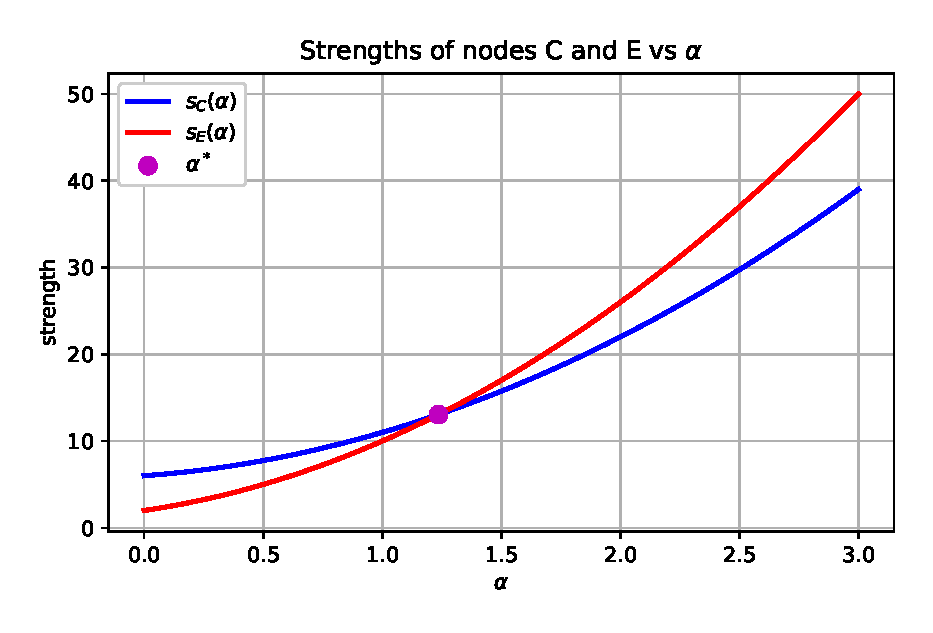
\includegraphics[width = .5\textwidth]{p3hw_figure_1.eps}
\end{center}
\caption{A plot of $s_C(\alpha)$ and $s_E(\alpha)$, which intersect at the critical value $\alpha = -1 + \sqrt{5} \approx 1.24.$ }
\label{quadratics}
\end{figure}

\item Confirm numerically the value of $\alpha$ you found in part (c) by using \verb|root_scalar| to find the intersection of $s_C(\alpha)$ and $s_E(\alpha)$.  \\

Python returns a critical $\alpha$ value of 1.2360679774997896, which is a good numerical approximation to $-1 + \sqrt{5}$.  


\item Modify the function \verb|plot_weighted_graph| to plot the weighted graph $A(\alpha)$ by introducing another input $A_{medium}$.  Plot the graph of $A(0.5)$ and include it in the \LaTeX\,report below. \\

The graph for $A(0.5)$ is provided in Figure \ref{graph} below.  We can see that the edge connecting nodes $A$ and $B$ is the strongest and the node connecting $A$ and $E$ is the weakest.  


\begin{figure}[b!]
\begin{center}
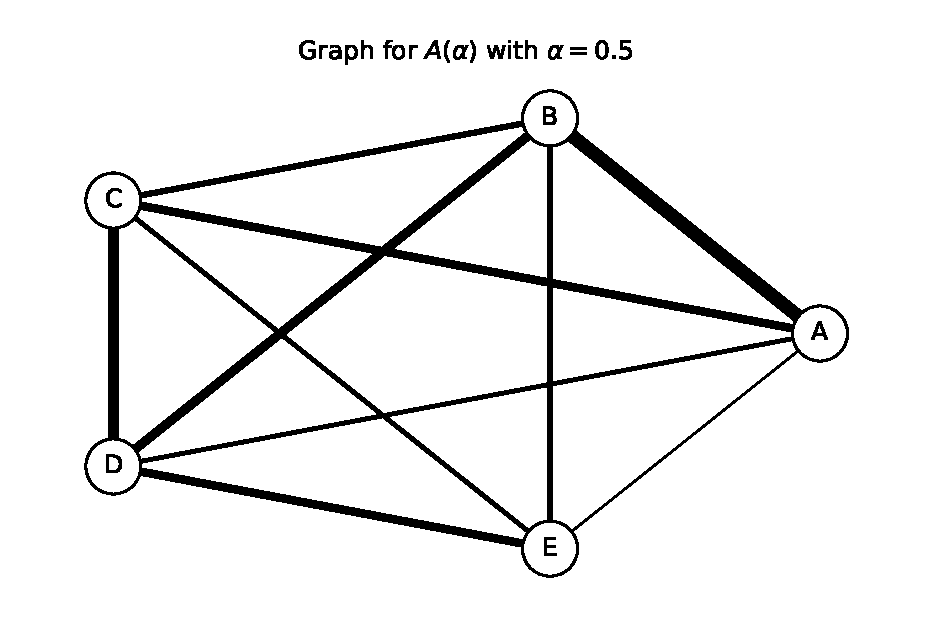
\includegraphics[width = .5\textwidth]{p3hw_figure_2.eps}
\end{center}
\caption{A depiction of the graph given by $A(0.5)$.   }
\label{graph}
\end{figure}


\end{enumerate}



\end{parts}

\pagebreak

%%%%%%%%%%%%%%%%%%%%%%%%%%%%%%%%%%%%%%
% NUMBER 3
%%%%%%%%%%%%%%%%%%%%%%%%%%%%%%%%%%%%%%
\question Consider the undirected graph $G$ with vertex set
\[ V=\{A,B,C,D,E,F\} \]
and edge set
\[ E=\{AB,AC,BC,BD,CE,DE,DF,EF\}. \]

\begin{parts}
\part Use Python to plot this graph and include it below.   \\ 

\begin{figure}[h!]
\begin{center}
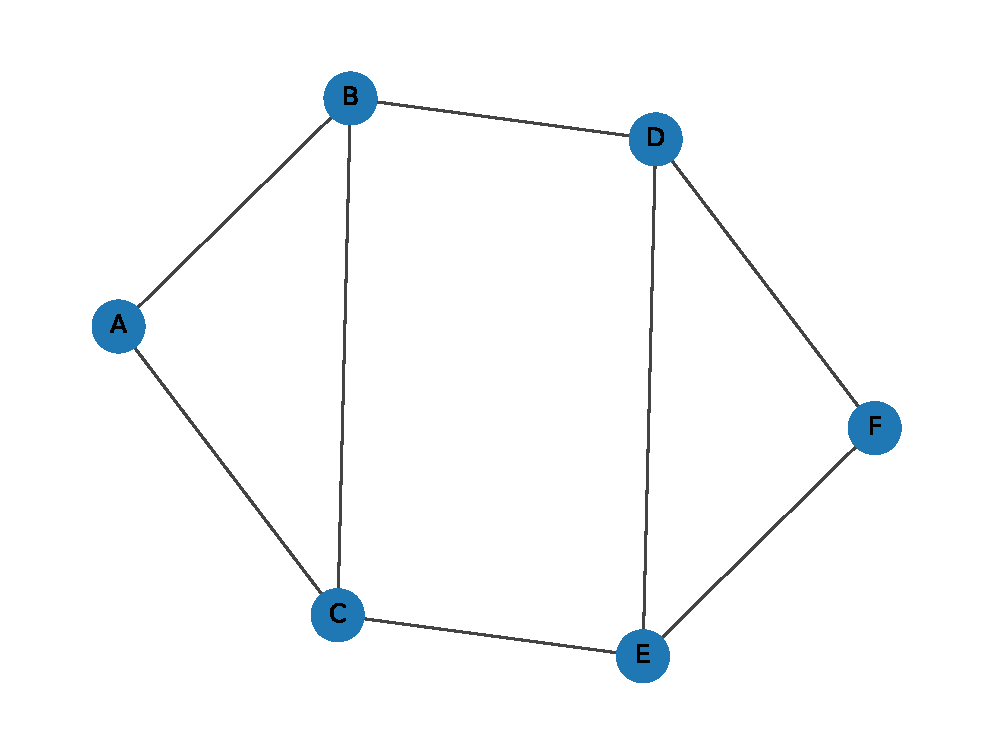
\includegraphics[width = .5\textwidth]{p3hw_figure_3.eps}
\end{center}
\caption{A depiction of the graph given by the vertex set $V$ and edge set $E$.   }
\label{graph}
\end{figure}


\part In the same Python file, compute the closeness, betweenness, and eigenvector centrality.  Include them all below and comment on if they agree.  Which node is the ``most important?"  \\ 

The three measures of centrality of each node is included in Table \ref{centrality} below.  

\begin{table}[h!]
\caption{Centrality scores for each node using three methods: closeness, betweenness, and eigenvector.}
\begin{center}
\begin{tabular}{ccc}
Closeness Centrality & Betweenness Centrality & Eigenvector Centrality \\\hline
A: 0.5556 & A: 0.0 & A: 0.3251 \\
B: 0.7143 & B: 0.2 & B: 0.4440 \\
C: 0.7143 & C: 0.2 & C: 0.4440\\
D: 0.7143 & D: 0.2 & D: 0.4440 \\
E: 0.7143 & E: 0.2 & E: 0.4440\\
F: 0.5556 & F: 0.0 & F: 0.3251 \\
\end{tabular}
\end{center}
\label{centrality}
\end{table}

We can see that the actual numerical values for each node is different for each 



\end{parts}

\end{questions}
\end{document}